% This file was created by matlab2tikz.
%
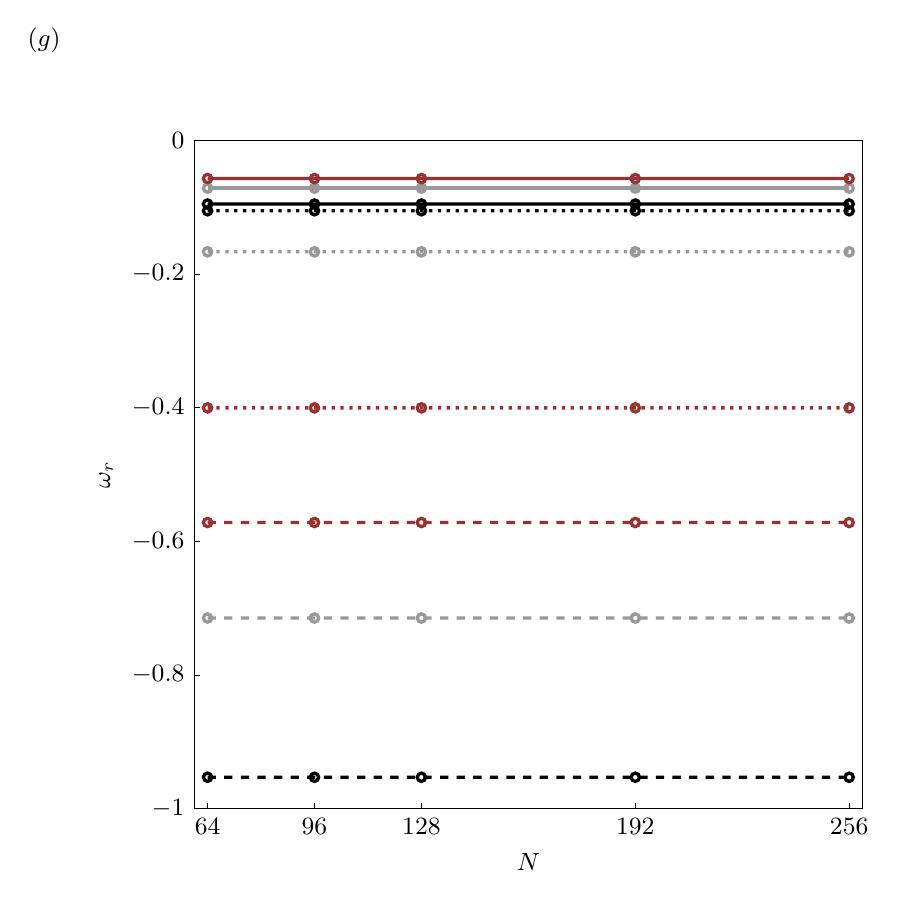
\begin{tikzpicture}

\begin{axis}[%
width=11.255in,
height=7.131in,
at={(1.888in,0.962in)},
scale only axis,
clip=true,
separate axis lines,
every outer x axis line/.append style={black},
every x tick label/.append style={font=\color{black}},
every x tick/.append style={black},
xmin=60,
xmax=260,
xtick={ 64,  96, 128, 192, 256},
xlabel={$N$},
every outer y axis line/.append style={black},
every y tick label/.append style={font=\color{black}},
every y tick/.append style={black},
ymin=-1,
ymax=0,
ylabel={$\omega_r$},
axis background/.style={fill=white},
clip=true,
clip mode=individual,
axis lines=box,
xtick pos=bottom,
ytick pos=left,
tick align=inside,
major tick length=2pt,
width=0.7\linewidth,
height=0.7\linewidth,
every axis/.append style={font=\fontsize{9}{9}\selectfont},xlabel style={font=\fontsize{9}{9}\selectfont},title style={font=\fontsize{9}{9}\selectfont},
legend style={font=\fontsize{8}{9}\selectfont,inner sep=1pt,row sep=1pt,column sep=2pt,nodes={scale=1.00},draw=none},legend image post style={xscale=0.35},
legend columns=1,
scaled x ticks=false,
tick label style={/pgf/number format/fixed,/pgf/number format/precision=2},
every x tick label/.append style={font=\fontsize{9}{9}\selectfont\color{black}},
every y tick label/.append style={font=\fontsize{9}{9}\selectfont\color{black}},
,,
colormap={sigmamap}{rgb(0.0000)=(0.0200,0.1880,0.3800); rgb(0.1000)=(0.0743,0.3456,0.5616); rgb(0.2000)=(0.1918,0.4980,0.7060); rgb(0.3000)=(0.3890,0.6708,0.8226); rgb(0.4000)=(0.7552,0.8682,0.9228); rgb(0.5000)=(0.9690,0.9689,0.9689); rgb(0.6000)=(0.9425,0.8044,0.7614); rgb(0.7000)=(0.8767,0.4910,0.4020); rgb(0.8000)=(0.7869,0.2866,0.2470); rgb(0.9000)=(0.6186,0.1239,0.1568); rgb(1.0000)=(0.4040,0.0000,0.1220)}
]
\addplot [color=black, line width=1.2pt, mark size=1.5pt, mark=o, mark options={solid, black}, forget plot]
  table[row sep=crcr]{%
64	-0.0952983983829359\\
96	-0.0952982646972484\\
128	-0.0952982606997138\\
192	-0.0952982606772919\\
256	-0.0952982606773163\\
};
\addplot [color=black, dashed, line width=1.2pt, mark size=1.5pt, mark=o, mark options={solid, black}, forget plot]
  table[row sep=crcr]{%
64	-0.952964518941961\\
96	-0.952963251202302\\
128	-0.952963213095514\\
192	-0.952963212882\\
256	-0.95296321288197\\
};
\addplot [color=black, dotted, line width=1.2pt, mark size=1.5pt, mark=o, mark options={solid, black}, forget plot]
  table[row sep=crcr]{%
64	-0.105330018827117\\
96	-0.105329870810532\\
128	-0.105329866364215\\
192	-0.105329866339398\\
256	-0.10532986633925\\
};
\addplot [color=white!60!black, line width=1.2pt, mark size=1.5pt, mark=o, mark options={solid, white!60!black}, forget plot]
  table[row sep=crcr]{%
64	-0.0714737354158967\\
96	-0.0714737071023862\\
128	-0.0714737041562195\\
192	-0.0714737041395548\\
256	-0.0714737041396149\\
};
\addplot [color=white!60!black, dashed, line width=1.2pt, mark size=1.5pt, mark=o, mark options={solid, white!60!black}, forget plot]
  table[row sep=crcr]{%
64	-0.714732576305744\\
96	-0.714731584987193\\
128	-0.714731555525715\\
192	-0.714731555360003\\
256	-0.714731555359999\\
};
\addplot [color=white!60!black, dotted, line width=1.2pt, mark size=1.5pt, mark=o, mark options={solid, white!60!black}, forget plot]
  table[row sep=crcr]{%
64	-0.166773147686156\\
96	-0.166772925362327\\
128	-0.166772918420891\\
192	-0.166772918384189\\
256	-0.166772918384776\\
};
\addplot [color=red!60!teal, line width=1.2pt, mark size=1.5pt, mark=o, mark options={solid, red!60!teal}, forget plot]
  table[row sep=crcr]{%
64	-0.0570976250939065\\
96	-0.0571790070619081\\
128	-0.0571790113729609\\
192	-0.0571790116053394\\
256	-0.0571790116052954\\
};
\addplot [color=red!60!teal, dashed, line width=1.2pt, mark size=1.5pt, mark=o, mark options={solid, red!60!teal}, forget plot]
  table[row sep=crcr]{%
64	-0.571781851480997\\
96	-0.571786395657606\\
128	-0.571786364055038\\
192	-0.571786364239759\\
256	-0.571786364240081\\
};
\addplot [color=red!60!teal, dotted, line width=1.2pt, mark size=1.5pt, mark=o, mark options={solid, red!60!teal}, forget plot]
  table[row sep=crcr]{%
64	-0.400249602068264\\
96	-0.400255735287743\\
128	-0.400255711515608\\
192	-0.400255712077295\\
256	-0.400255712071431\\
};
\node[right, align=left, inner sep=0]
at (rel axis cs:-0.25,1.15) {$(g)$};
\end{axis}
\end{tikzpicture}%